\section{Clothing Image Preprocessing}

\subsection{Overview}
In order to train a small CNN model that is capable of classifying clothing images accurately, it's essential that our training data contains just sufficient information about the clothing but without much noise. However, the clothing image dataset usually include the background and a model, which bring in lots of noisy information and could seriously degrade the performance of our classifier. Therefore, to minimize such noise and unify the data format of the clothing images, we preprocess the clothing dataset to extract a $128 \times 128$ block out of each image, which contains the clothing object only.

The preprocessing process is as follows, for each image, a salient object detection algorithm is first applied to detect the region containing the most salient object, then the detected region is cropped and resized to $128 \times 128$ pixels. Since our model is only concerned about the shape of clothing object for classification, we further convert the extracted block into grayscale. In the end, to make the training easier, the pixel value is normalized to have a mean of 0 and standard deviation of 0.5 approximately. In all, the final output of the preprocessing for an image is a $128 \times 128$ matrix of float values in range $[-0.5,  0.5]$.

\subsection{FASA Object Detection}
In this project, the \emph{FASA object detection} algorithm developed by Yildirim G{\"o}khan et al. \cite{yildirim2014fasa} is adopted for salient objection detection. Compared to other state-of-art object detection algorithm, FASA distinguishes itself by satisfying both accuracy and efficiency. It's shown that FASA is one order of magnitude faster than other methods emphasize on accuracy and still have comparable accuracy.

The FASA method combines a probability of saliency with a global contrast map. To achieve efficiency, it first perform a color quantization and forms a histogram in CIEL*a*b color space. Then the spatial center and variance of each quantized color is calculated for estimating the position and size of the salient object and computing the probability of saliency. The quantized color are also used to generate a global color contrast value. In the end, the saliency probability and color contrast value are fused to generate a saliency map, which maps each pixel in the image to a saliency value. Running the FASA algorithm against an image can produce $k$ bounding areas with corresponding saliency values, where k is the number of quantized color.

In this project, we only want to detect one salient object within each clothing image, therefore, only the bounding area with highest salient value is selected and extracted as described above.

\subsection{Preprocessing Result}
This subsection shows the result of preprocessing.
\begin{figure}[h]
  \centering
  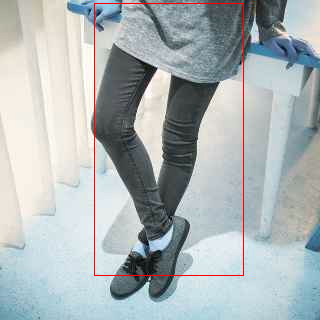
\includegraphics[width=0.8\columnwidth]{box}
  \caption{An image of a nice gray jean}
  \label{fig:sample_image}
\end{figure}

Figure \ref{fig:sample_image} shows a model wearing the gray jean, in this case, the jean is our interested object. By applying the FASA algorithm, the bounding region shown in the figure is detected.

\begin{figure}[h]
  \centering
  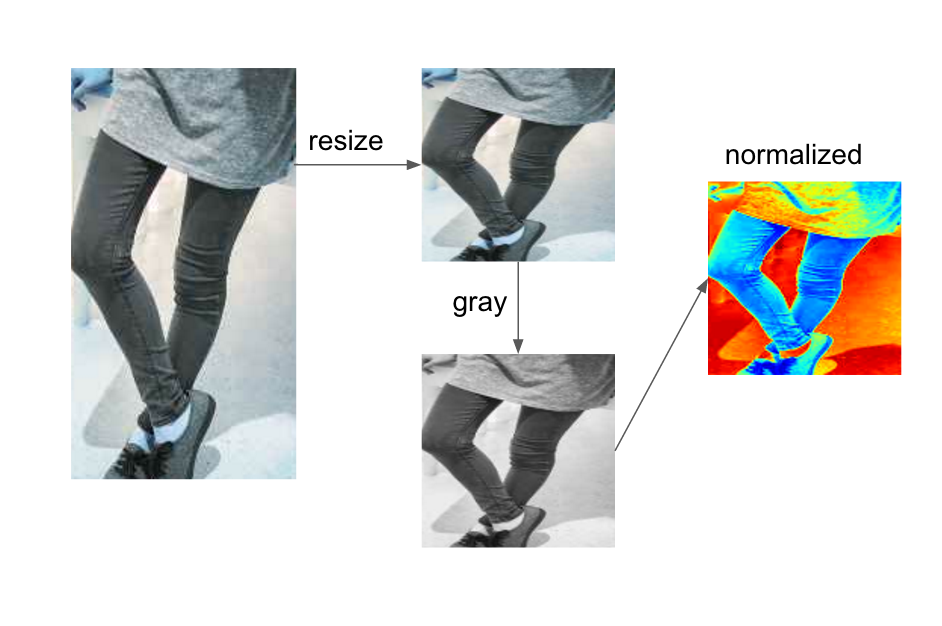
\includegraphics[width=0.9\columnwidth]{normalized}
  \caption{The preprocessing flow of one image}
  \label{fig:normalized}
\end{figure}

Following the process described above, the detected region is cropped out and resized into $128 \times 128$ pixels, and then converted into grayscale. The pixel value of the resulted image is further normalized into float-point values within $[-0.5, 0.5]$, the last image in Figure \ref{fig:normalized} shows that the image is still discernible after normalization.
